\documentclass[../tesis_main.text]{subfiles}

\chapter{Detección de objetos}
En este capítulo se trata el desarrollo de los algoritmos propuestos en la metodología de este trabajo. Se comenzará con los desarrollos realizados en el ámbito de la visión computacional:\\

	\begin{itemize}
		\item{Segmentación de planos}
		\item{Extracción de planos}
		\item{Segmentación de objetos}
		\item{Cálculo del centroide de un objeto}
		\item{Aproximación a la orientación de un objeto}
	\end{itemize}

	Posteriormente se abordarán los temas respectivos la cinemática de un brazo robótico de 7DOF. En este apartado abordaremos la cinemática directa del mismo y como trabajo futuro queda la cinemática inversa del mismo.\\

	Es importante mencionar que los desarrollos reportados en este trabajo fueron realizados en el framework para el desarrollo de software para robots, ROS por sus siglas en inglés. Alojado en el sistema operativo Ubuntu.\\

	%**Acondicionamiento de Nube de puntos(???) Transformaciones(???)

	\section{Segmentación de planos con RANSAC}

		Para el desarrollo del algoritmo RANSAC se utilizó el sensor Kinect dado que este sensor, además de una imagen de color, proporciona información sobre la profundidad de los objetos. Con un manejo adecuado de ambos datos se pueden conseguir avances notables en el campo de la visión computacional.\\

		Para el desarrollo del algoritmo se hizo uso de la información de profundidad de los objetos.\\

		\begin{figure}[h!]
			\begin{center}
			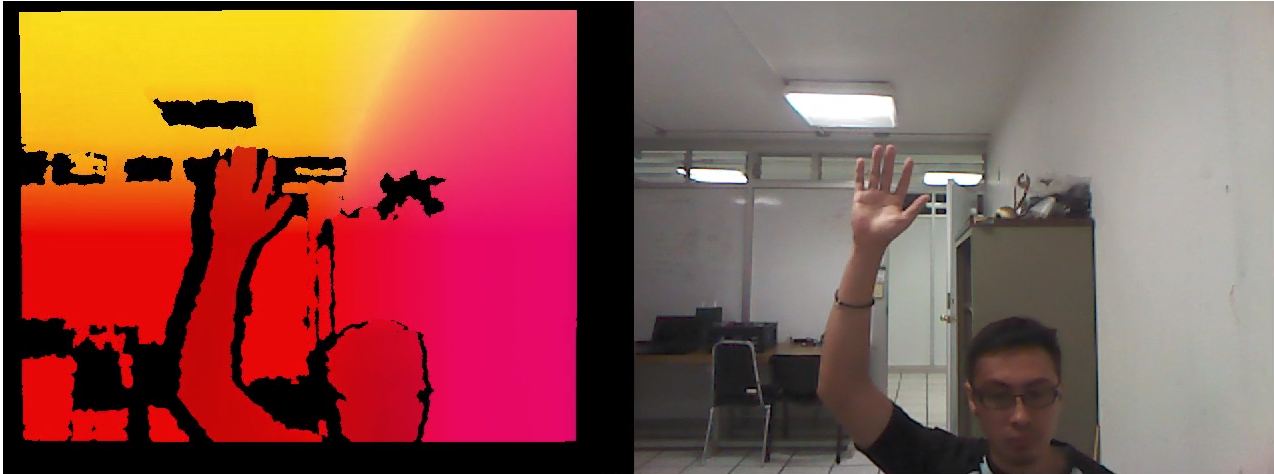
\includegraphics[width=10.5cm, height=4.5cm]{vision/pointCloud1.png}	
			\caption{Imagen típica de la información otorgada por el sensor Kinect.}
			\end{center}
		\end{figure}
		
		Se desarrolló un programa en lenguaje C++ para segmentar los planos. La información de profundidad entregada por el Kinect, se da en una matriz donde cada elemento $i, j$ contiene la información de profundidad obtenida por el sensor, como se muestra a continuación:\\

		%%***imagen de matriz profundidad (talvez estrecha)\\

		Cada elemento de la matriz contiene información de un punto $p = (x, y, z)$ donde el haz infrarojo fue reflejado, esto nos permite conocer la distancia a la cual se encuentra un objeto, o su superficie. La información que nos entrega el sensor en forma de matriz es de dimensiones $640 x 480$ por tanto consta de 307,200 elementos en total.  Dentro de este conjunto de datos procura encontrar las superficies planas.\\

		Se programó el algoritmo RANSAC para extraer planos en C++, el código se puede consultar en la página. ***(github ref).\\

		Para la correcta implementación del algoritmo fue necesario tomar algunas consideraciones, por ejemplo: descartar del procesamiento todos aquellos píxeles que no proporcionen información relevante de profundidad, la construcción de una clase para generar planos.\\

		Para la construcción de planos se tomaron tres puntos aleatorios y se construyeron dos vectores a partir de los puntos y se realizó el producto cruz entre estos.\\ 

		\begin{center}
			$p_1 = rnd(datos)$\\
			$p_2 = rnd(datos)$\\
			$p_3 = rnd(datos)$\\

			$\vec{v_1} = p_1 - p_2$\\
			$\vec{v_2} = p_1 - p_3$\\

			$\vec{N} = \vec{v_1} \times \vec{v_2}$
		\end{center}

		Conocemos la ecuación general del plano:\\

		 $\Pi: Ax + By + Cz + D = 0$\\

		donde: A, B, C son las componentes del vector normal respectivamente y D la podemos calcular como:\\

		$D = (A*p_1.x + B*p_1.y + C*p_1.z)$ \\

		Por lo tanto con tres puntos seleccionados aleatoriamente tenemos un modelo de plano generado aleatoriamente. Lo cual es el primer requerimiento para el algoritmo.\\ 

		Posteriormente se comparó el resto de la información con ese modelo propuesto aleatoriamente y verificamos que tan buen modelo es. Para ello calculamos la distancia euclidiana de cada punto al plano propuesto, si la distancia es menor que cierto umbral lo consideramos como parte del modelo e incrementamos el numero de puntos que empatan con el modelo \"inliers\".\\

		Del mismo modo se buscaba que el numero de inliers que empataran con el modelo fuera al menos el 60\% del total de datos. En los resultados se trata este tema con mayor profundidad.\\

		Observamos que el algoritmo opera bien con un numero máximo de iteraciones = 70, y con un umbral de error de 2 cm.\\


		\begin{figure}[h!]

			\begin{subfigure}[t]{.5\textwidth}
			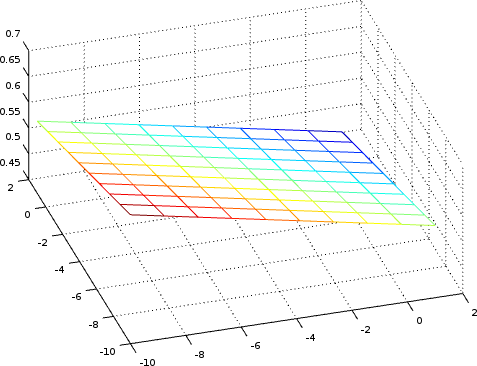
\includegraphics[width=5.5cm, height=3.0cm]{planes/plane.png}	
			\caption{Grafico de un plano en tercera dimensión.}
			\end{subfigure}%
			\begin{subfigure}[t]{.5\textwidth}
			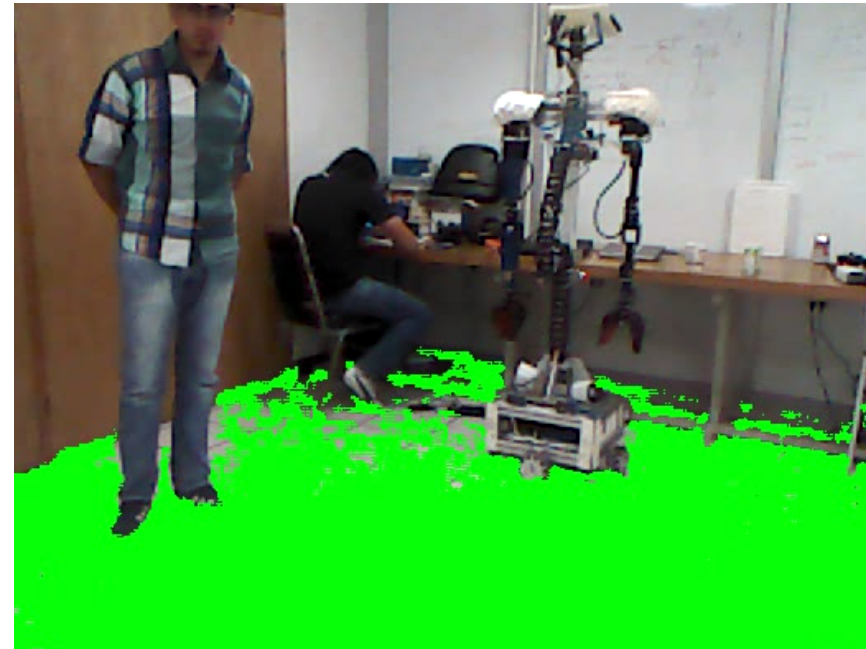
\includegraphics[width=6.5cm, height=3.0cm]{planes/planeSegmentation5.png}
			\caption{Segmentación de un plano utilizando el sensor kinect.}
			\end{subfigure}

			\caption{Planos y su representación en 3D.}
		\end{figure}


		Por ahora el algoritmo no restringe su búsqueda a planos horizontales o verticales, quedá como trabajo futuro el desarrollo de una búsqueda selectiva de planos con características similares a una mesa, destacando características de horizontalidad y altura.\\


	\section{Extracción de objetos}
		
		Una vez  que se encontró la nube de puntos perteneciente al modelo, se prosiguió a ubicar espacialmente los objetos que se encontraban sobre el plano. Se realizó la extracción de objetos con las siguientes restricciones:\\

		\begin{itemize}
			\item{$ p_n = null$   $\forall$  $p_n \in \Pi$ }
			\item{$ p_n = null$   $\forall$  $p_n.z < Height(\Pi)  $ }
			\item{$ p_n = null$   $\forall$  $p_n.x > 0.50[m]  $ }
		\end{itemize}

		De otro modo esto sería igual a:\\

		\begin{itemize}
			\item{Extracción de los puntos pertenecientes al plano.}
			\item{Extracción de los puntos por debajo del plano.}
			\item{Extracción de los puntos más allá de 40 respecto al punto más cercano en x.}
		\end{itemize}

		\begin{figure}

			\begin{subfigure}[h]{.5\textwidth}
			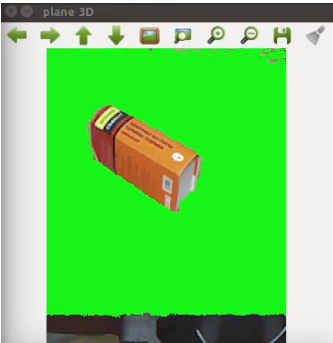
\includegraphics[width=5.5cm, height=4.0cm]{objs/object1.png}	
			\caption{Extracción del color objeto.}
			\end{subfigure}%
			\begin{subfigure}[h]{.5\textwidth}
			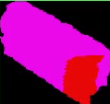
\includegraphics[width=4.5cm, height=3.5cm]{objs/object1_pc.png}
			\caption{Información de profundidad del objeto.}
			\end{subfigure}

			\caption{Extracción de información del objeto.}
		\end{figure}

		Posterior a este proceso tenemos como resultado un conjunto de puntos reflejados sobre un objeto sólido con las distancias proyectadas sobre los tres ejes coordenados respecto del robot Justina.\\


	\section{Aproximación de orientación de objetos con PCA}

		El análisis de componentes principales se usa abundantemente en muchas formas de análisis de datos. En este caso se utilizará como una metodología para reducir un conjunto de datos a una dimensión inferior. Más concretamente la forma en que podemos obtener una base ortogonal del conjunto de datos, que represente la distribución de los puntos proyectados sobre el objeto. Esta base, representará la dirección de la distribución de los puntos del objeto, y por tanto encontraremos la dirección del objeto mismo respecto al robot.\\  

		\subsection{Adquisición de datos y cálculo de la media}
			La adquisición de datos se realizó mediante la extracción de los puntos pertenecientes al objeto. Cada uno de los datos perteneciente al conjunto de puntos posee tres características:\\

			\begin{itemize}
				\item{La distancia al objeto  proyectada sobre el eje $x$}
				\item{La distancia al objeto  proyectada sobre el eje $y$}
				\item{La distancia al objeto  proyectada sobre el eje $z$}
			\end{itemize} 

			Por lo tanto, de una nube de puntos como la mostrada en la figura () podemos extraer medidas de dispersión, y medidas de tendencia central. Se partió con el cálculo de la media de los datos. $\bar{X}, \bar{Y}, \bar{Z}.$ El punto $P(\bar{X}, \bar{Y}, \bar{X})$ representa el centroide del objeto. Conociendo este punto podemos conocer la ubicación espacial del objeto respecto del robot y determinar si es manipulable (si se encuentra dentro del área de trabajo) y conocer las coordenadas a donde deberíamos llevar el efector final de nuestro manipulador para manipularlo.\\

			Para realizar el cálculo de la media se cuantifico el número de puntos pertenecientes al objeto, $(n)$. Posteriormente, para todos los puntos pertenecientes al conjunto $n$ se sumaron sus valores en $\bar{X}, \bar{Y}, \bar{Z}$, respectivamente. Y posteriormente se dividieron entre $n$.\\

			\noindent\fbox
			{
			\begin{minipage}{1.0\textwidth}\small
			\begin{algorithmic}
		

				    \For{ cada punto \textbf{in} datos}
				    	\State{$X_{total} = X_{total} + dato_{x}$}
				    	\State{$Y_{total} = Y_{total} + dato_{y}$}
				    	\State{$X_{total} = X_{total} + dato_{z}$}
				    \EndFor{}\\
				    	\State{$\bar{X} = \dfrac{X_{total} } {n} $}\\
				    	\State{$\bar{Y} = \dfrac{Y_{total} } {n} $}\\
				    	\State{$\bar{X} = \dfrac{X_{total} } {n} $}\\

				\State{\textbf{return} $P(\bar{X}, \bar{Y}, \bar{Z})$}
			\end{algorithmic}
			
			\end{minipage}
			}

			%%Ïmagen centroides Rviz.
			\begin{figure}[h!]

				\begin{subfigure}[h]{.5\textwidth}
				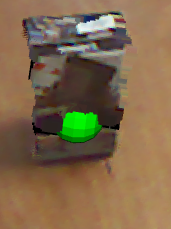
\includegraphics[width=3.5cm, height=5.0cm]{objs/centroid3.png}	
				\end{subfigure}%
				\begin{subfigure}[h]{.5\textwidth}
				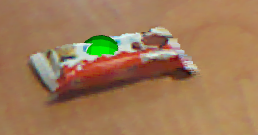
\includegraphics[width=6.0cm, height=3.5cm]{objs/centroid5.png}
				\end{subfigure}
			
			\caption{Segmentación de un objeto y su correspondiente centroide (punto verde).}

			\end{figure}
			

		\subsection{Cálculo de la matriz de covarianza}
			Dada una variable estadística n-dimensional  $(X_1, X2,X3,...,Xn)$, llamaremos matriz de covarianzas a la matriz cuadrada, $n \times n$, que disponga en su diagonal principal de las varianzas de cada una de las distribuciones marginales unidimensionales, y en los elementos no-diagonales $(i,j)$ de las correspondientes covarianzas entre cada dos variables $S_{ij}.$\\

			Para ello se hizo uso de las expresiones matemáticas correspondientes:\\

			 \begin{equation}
				\begin{split}
					var(X) = \dfrac{\Sigma^n_{i=1} (X_i - \bar{X} ) (X_i - \bar{X}) } { n }
				\end{split}
			\end{equation}

			\begin{equation}
			\begin{split}
				cov(X, Y) = \dfrac{\Sigma^n_{i=1} (X_i - \bar{X} ) (Y_i - \bar{Y}) } { n }
			\end{split}
			\end{equation}

			A continuación se anexa en código correspondiente al cálculo de las varianzas y covarianzas.\\



			\begin{lstlisting}[language=c++, caption=Cálculo de varianzas y covarianzas]
//Calculate covariance matrix
for(int j = 0; j < object.rows; j++)
	for (int i = 0; i < object.cols; i++)
	{
		px = object.at<cv::Point3f>(j,i);
		if ( px != cv::Point3f(0.0, 0.0, 0.0) && px != cv::Point3f(0, 255, 0))
		{
			var_x += pow( (px.x - centroid[0]), 2 );
			var_y += pow( (px.y - centroid[1]), 2 );
			var_z += pow( (px.z - centroid[2]), 2 );
			cov_xy += ( px.x - centroid[0] )*( px.y - centroid[1] );
			cov_xz += ( px.x - centroid[0] )*( px.z - centroid[2] );
			cov_yz += ( px.y - centroid[1] )*( px.z - centroid[2] );
			n++;
		}
	}

var_x /= n;
var_y /= n;
var_z /= n;

cov_xy /= n;
cov_xz /= n;
cov_yz /= n;

cov_matrix << var_x,  cov_xy, cov_xz,
				 cov_xy,  var_y, cov_yz,
				 cov_xz, cov_yz,  var_z;
			\end{lstlisting}

			Posteriormente se propuso a encontrar los valores de los vectores propios asociados a la matriz de covarianzas. En la literatura existen múltiples métodos numéricos para la solución de esta problemática, como la puesta a prueba de dichos algoritmos no es el propósito de este trabajo se optó por utilizar la librería \textbf{eigen}. Por tanto, una vez construida la matriz de covarianzas M, se utiliza la instrucción:\\

			\begin{lstlisting}[language=c++, caption=Cálculo de varianzas y covarianzas]
Eigen::SelfAdjointEigenSolver<Eigen::MatrixXf> eig(cov_matrix);
			\end{lstlisting}

			La instrucción \textit{Eigen::SelfAdjointEigenSolver<Eigen::MatrixXf>} nos devuelve un objeto \textit{eig} cuyos atributos son \textit{eigenvalues()} y \textit{eigenvectors()}. Con ayuda de esta librería podemos obtener fácilmente los eigenvectores de la matriz M. Es importante mencionar que el atributo \textit{eigenvectors()} del objeto \textit{eig} se encuentra normalizado; por lo tanto es conveniente darle un escalamiento relacionado con la dispersión de los datos. De este modo se optó por multiplicar cada uno de los eigenvectores por su correspondiente valor de desviación estándar.\\

			\begin{figure}[ht!]

				\begin{subfigure}[h]{.5\textwidth}
				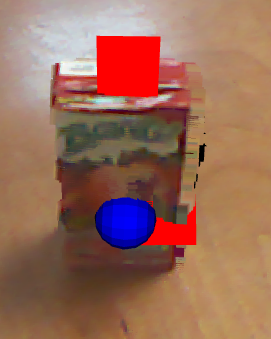
\includegraphics[width=3.5cm, height=5.0cm]{objs/centroid_1.png}	
				\end{subfigure}%
				\begin{subfigure}[h]{.5\textwidth}
				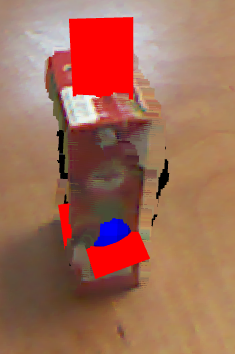
\includegraphics[width=3.5cm, height=5.0cm]{objs/centroid2.png}
				\end{subfigure}
			
			\caption{Segmentación de un objeto y sus correspondientes ejes principales (rojo).}

			\end{figure}